% !TEX TS-program = pdflatexmk
\documentclass{styles/assisi}
\DeclareRobustCommand{\DelivNumber}{CATS2.0 architecture}
\DeclareRobustCommand{\DelivName}{\today}
\DeclareRobustCommand{\DelivStatus}{Confidential}
\DeclareRobustCommand{\DelivRevision}{0.1}
\DeclareRobustCommand{\DeliveryDate}{}
\DeclareRobustCommand{\DelivPartnersOwning}{\bf EPFL}
\DeclareRobustCommand{\DelivPartnersContributing}{\bf PARIS7}
\DeclareRobustCommand{\DelivPartnersContributingNextLine}{}
\DeclareRobustCommand{\DelivDue}{M6}
\DeclareRobustCommand{\DelivAbstract}{This report summarises ongoing work in ASSISI regarding the development of CASUs and the VRRI-System.}

%----------------------------------------------------------------------------------------------
\makeindex

\usepackage{epsfig,subfigure,float,pseudocode,multirow,footmisc,rotating}
\usepackage{graphicx}        % standard LaTeX graphics tool
\usepackage{amsmath, amssymb, subfigure}
\usepackage{multirow, rotating}
\usepackage[ruled,lined,commentsnumbered]{algorithm2e}
\usepackage[colorlinks=false, urlcolor=blue, pdfborder={0 0 0}]{hyperref}
%\usepackage{algorithm2e}
\usepackage{pdfpages}
\usepackage{afterpage}
\usepackage{booktabs}
\usepackage{listings}

\newcommand{\rd}{\Delta^{\frac{1}{2}}}
\newcommand{\pla}{\phi_{\lambda_1}^t}
\newcommand{\plb}{\phi_{\lambda_2}^t}
\newcommand{\ie}{i.\,e.,\ }
\newcommand{\Ie}{I.\,e.,\ }
\newcommand{\eg}{e.\,g.,\ }
\newcommand{\Eg}{E.\,g.,\ }
\newcommand{\assisi}{ASSISI$|_{bf}$ }
\setcounter{tocdepth}{3}

% TODO command
\newcommand{\todo}[1]{\par\noindent{\raggedright\textsc{\color{red}#1}%
    \par\marginpar{{\Large\color{red}$\star$}}}}

\begin{document}
\thispagestyle{plain}
  \vspace*{0.3cm}
  \begin{center}
  {\bf \LARGE SEVENTH FRAMEWORK PROGRAMME}\\
  \vspace*{0.6cm}
  
\includegraphics[width=0.15\textwidth]{styles/7th.png}\\
  \vspace*{2.0cm}
  \bf {\large IP}\\
  \vspace*{1.0cm}
  \bf {\Huge ASSISIbf}\\
  \vspace*{.6cm}
  \bf {\it \Large Animal‌ and‌ robot‌ Societies‌ ‌Self-organise‌ and‌ Integrate‌ by‌ Social‌ Interaction‌ (bees‌ and‌ fish)‌}\\
  \vspace*{45pt}
  {\huge \bf \DelivNumber}\\
  \vspace*{12pt}
  {\Large \it \bf \DelivName}\\
  \vspace*{70pt}
  \small
  \begin{tabular}{|ll|}
    \hline &\\
    Date of preparation: \DeliveryDate & Revision: \DelivRevision\\ &\\
    Start date of project: February 1st, 2013 & Duration: 60 months\\ &\\
    Project co-ordinator: UNIGRAZ & Classification: \DelivStatus \\ &\\
    Partners: & \\
    %& \\
    ~~{\it owning:} \DelivPartnersOwning &~~{\it contributed:} \DelivPartnersContributing\\
    &\DelivPartnersContributingNextLine\\
    &\\
    Project website: & http://assisi-project.eu\\
    &\\
    \hline
  \end{tabular}
  \end{center}
%\newpage
%
%%-----------------------------------------------------------------
%\begin{center}
%\begin{tabular}{|lp{10cm}|}
%\hline &\\
%\multicolumn{2}{|c|}{\bf \Large DELIVERABLE SUMMARY SHEET} \\
%&\\
%\hline \hline
%&\\
%Project Number: & 601074\\
%&\\
%Project Acronym: & {\bf ASSISIbf}\\
%&\\
%Title:     & Animal‌ and‌ robot‌ Societies‌ ‌Self-organise‌ and‌ Integrate‌ by‌ Social‌ Interaction‌ (bees‌ and‌ fish) \\
%&\\
%\hline \hline
%&\\
%Deliverable N$^o$: & \DelivNumber\\
%&\\
%Due Date: & Project month: \DelivDue\\
%&\\
%Delivery Date: & \DeliveryDate \\
%&\\
%\hline \hline
%&\\
%\textbf{Name:} & {\bf \DelivName}\\
%&\\
%\textbf{Description:} & \DelivAbstract\\
%&\\
%&\\
%\hline \hline
%&\\
%Partners owning: & \DelivPartnersOwning \\
%&\\
%&\\
%Partners contributed: & \DelivPartnersContributing ~\DelivPartnersContributingNextLine \\
%&\\
%&\\
%Made available to: & \DelivStatus\\
%&\\
%\hline
%\end{tabular}
%\end{center}
%%}{}



%------------------------------------------------------------------



\textsf{\tableofcontents}
%\textsf{\listoffigures}
%\addcontentsline{toc}{chapter}{List of Figures}
%\textsf{\listoftables} \addcontentsline{toc}{chapter}{List
%of Tables}


\chapter{Introduction}\label{chap:intro}
\section{Tracking}
It has been always acknowledged in the life sciences that the problem of laborious and monotonous data analysis should be addressed by automation. By replacing a human observer with an intelligent system, we can avoid the variability in the human observation due to its intrinsic subjectivity. But, to be efficient, such systems have to be able to monitor continuous visual, acoustic and other displays to estimate various characteristics of animals and to detect behavioural events and patterns.

Animal behaviour is essentially related to movement; that is why a video recording becomes an irreplaceable tool for ethological research and documentation. The traditional way to analyze experimental video in ethology has always been through a manual marking of the positions of the animals on a video recording and a tagging of their behaviour, frame by frame at a given timescale. It is a tedious process that requires constant concentration, so a software that can automate or, at least, semiautomate it is highly welcomed.

\section{Robotic control}
In the robot-animal experimentation a robot might function autonomously relying only on its on-board sensors and computational resources. Alternatively the robot's control system might receive input information about robot's own state and states of other agents from the external sensors. Also the control system itself can be split on several levels of hierarchy, some running on-board and others on the external CPU controlling one or several robots (Fig. \ref{fig:overview}).

\begin{figure}[ht]
\centering
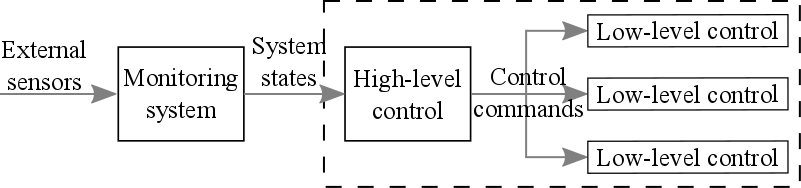
\includegraphics[width=0.75\textwidth]{./figs/overview.png}
\caption{The general overview of the animal-robot experimentation's monitoring and control system}
\label{fig:overview}
\end{figure}

\section{Retrospective}
A short overview of what was done for the automatization of the animal-robot experimentation in EPFL's Mobots group in collaboration with the University of Brussels and later with the University Paris 7.

\subsection{Chicken-robot project}
\subsubsection{Tracking}
We used two different approaches to track chicks : one solution for a real-time tracking and another for an off-line data analysis. For real-time tracking we used the SwisTrack software. Estimated robot position and orientation, chick positions and group parameters are transferred to the robot control system through the wireless radio connection.

\subsubsection{Control}
To build the control system of the PoulBot we used a behaviour based approach. Behaviour-Based systems work well in dynamic environments, in cases when fast reaction and high adaptability are important. These characteristics make the behaviour based approach a natural choice when designing a control system for a robot that interacts with animals. The control system of our robot is a hierarchical behaviour based controller. The robot is equipped with a set of primitive behaviours tightly bonded with the sensors and actuators of the robot. Each primitive behaviour serves to achieve a particular goal or to perform a specific activity. Examples of primitive behaviours are "wall-following", "emit-sound", "wall-avoidance", "goal-chasing", etc. These behaviours are executed on the microcontrollers of modules of PoulBot. The primitive behaviours are combined together to form higher level composite behaviours for specific experiments. The robot is provided with information about its position and positions of chicks by the external vision system through the wireless connection. Composite behaviours can run on the robot main board, or on the experimental PC (for debug and demonstration reasons).

\subsubsection{GUI}
The experimental PC runs a GUI interface of the PoulBot control system that allows the user to activate a specific behaviour and to specify its parameters (e.g., velocity, sensors thresholds, etc.). It also provides the user with the information on the status of the robot, such as battery charge level and current executed behaviour (Fig. \ref{fig:poulbot_control}, Fig. \ref{fig:poulbot_control_gui_settings}).

\begin{figure}[ht]
\centering
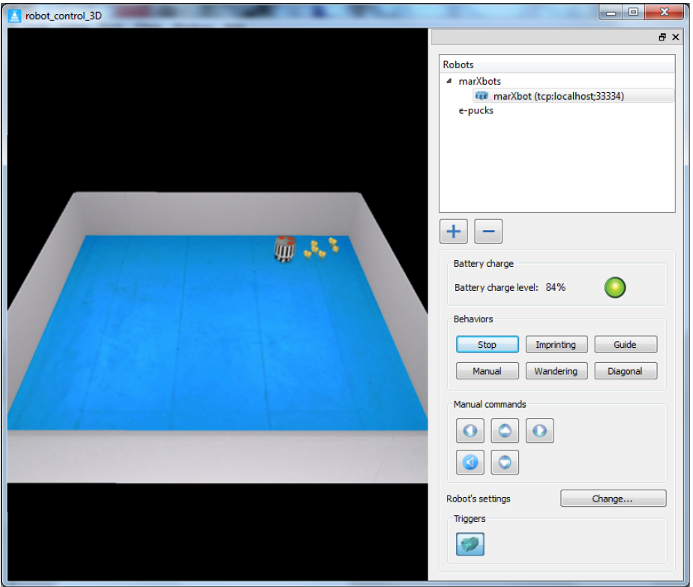
\includegraphics[width=0.75\textwidth]{./figs/poulbot_control_gui.png}
\caption{The graphical user interface of the PoulBot control system. On the left side is the virtual view of the experimental arena that receives data on robot's and chicks' positions from the external vision system, while on the right side is the list of connected robots and the control elements of the selected robot that allow the user to activate a specific  behaviour and to specify its parameters}
\label{fig:poulbot_control}
\end{figure}

\begin{figure}[ht]
\centering
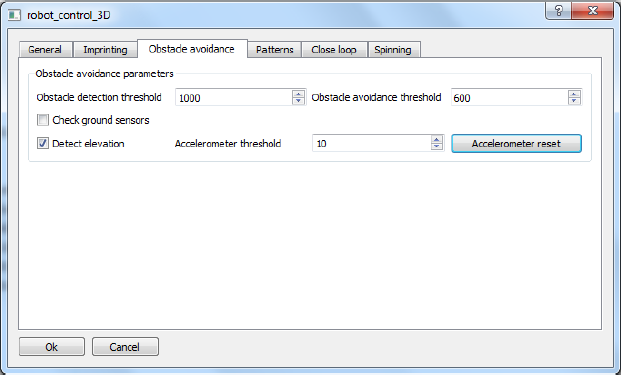
\includegraphics[width=0.65\textwidth]{./figs/poulbot_control_gui_settings.png}
\caption{The graphical user interface provides an access to parameters of robots behaviours such as speed, thresholds for different sensors, etc.; the parameters are logically grouped in several tabs.}
\label{fig:poulbot_control_gui_settings}
\end{figure}

\subsubsection{Monitoring}
To avoid bias in the behaviour of the animals, nobody is allowed to be in the experimental room while the experiments are running. To remotely observe a situation on the arena, we developed a lightweight and simple multi-platform remote viewer that connects to the SwisTrack through TCP/IP and provides a 3D representation of the arena. The data stream is coded by using the NMEA 0183 protocol; since only coordinates are transferred, the load on the network is considerably lower than if we would transfer a video stream. An additional
plug-in to this viewer was developed that automatically analyses the experimental situation to detect abnormal situations.

\subsubsection{OS}
All software was written in C++, relied on Qt for the user interface. It could run under Windows only due as the camera driver was available for Windows only.

\subsubsection{Software analysis}

PROS:
\begin{itemize}
  \item Several robots of various types (marXbot or ePuck) could be connected each one with its own controller
  \item Modularity of the solution
  \item Safety module
\end{itemize}

CONS:
\begin{itemize}
  \item External tracker was used, hence it was not possible to integrate the tracking and robotic control in a single application
\end{itemize}


\subsection{ASSISI project}
The Control And Tracking Software (CATS) was developed to track the positions of the agents, and to control the fish-CASUs. CATS is able to track the positions of both fishes and fish-CASUs in real-time. It is also able to differentiate a fish from a fish-CASU. Robot control makes use of the tracked positions of the fish-CASUs. 

\section{CATS}
The Control and Tracking Software (CATS) is designed to track the positions of the agents (fish and robots), and to control the fish-CASUs. Each robot can be controlled to display a collection of implemented behaviours. CATS's architecture was designed to be modular. It is composed of four parts, described in Fig. \ref{fig:CATS}. The first part manages the video stream from the camera of the experimental setup. The second part tracks the positions of fish and fish-CASUs. A Graphical User Interface (GUI) is provided to allow the experimenters to see the video stream, and to change the behaviour of the robots. The Control part contains implementations of the various behaviours and movement patterns of the fish-CASUs, and low-level methods to communicate with the fish-CASUs. Additionally, the system is designed to be easily integrable with analytical frameworks, like HEAF. It can be configured using the same configuration files as HEAF.

\afterpage{
\begin{figure}[ht]
\centering
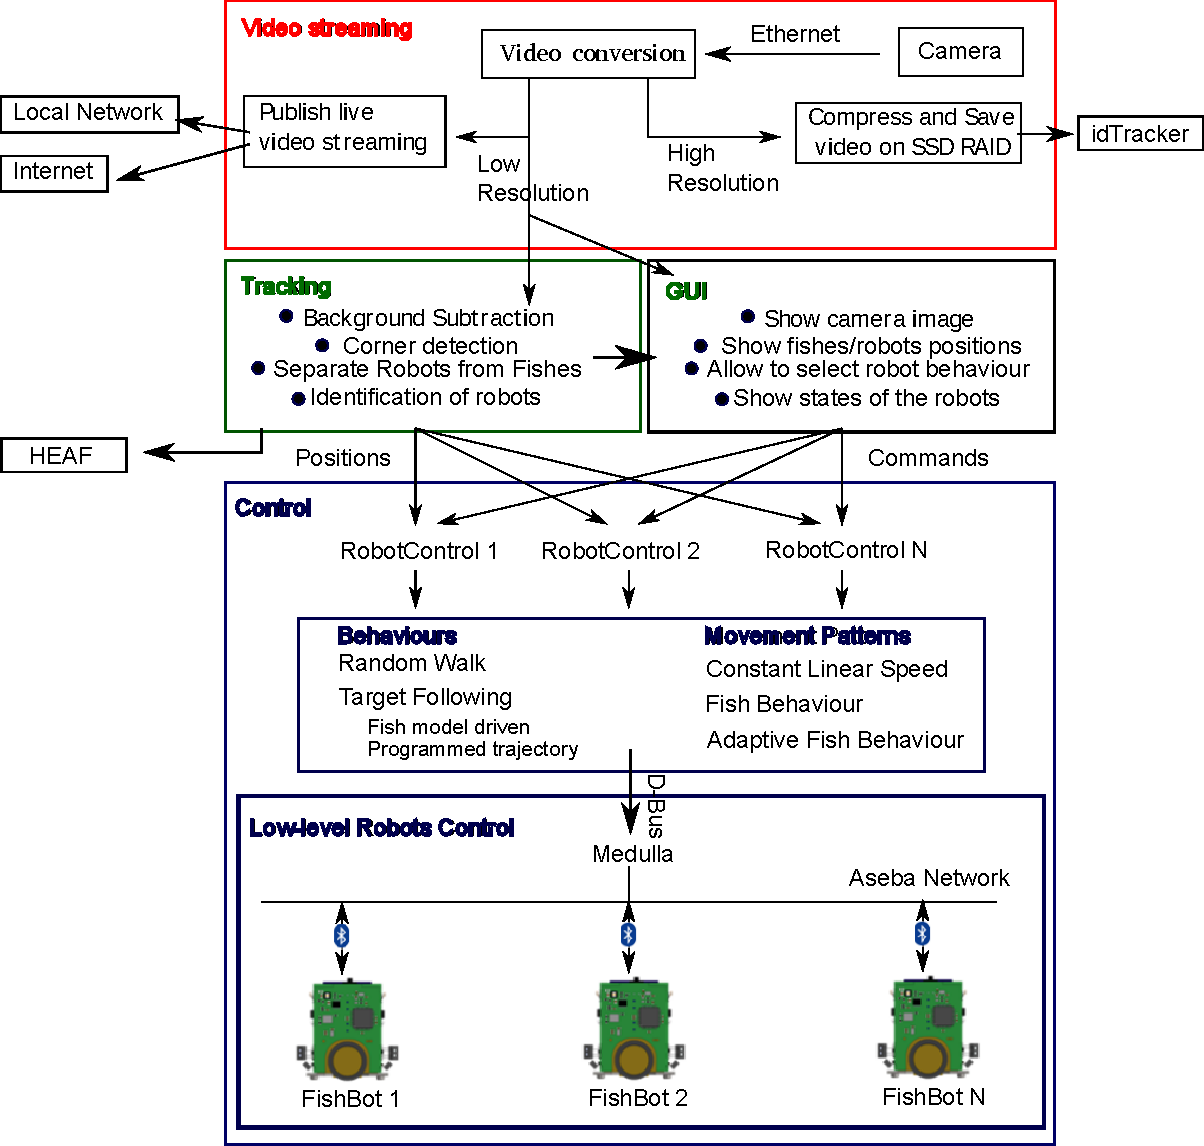
\includegraphics[width=0.8\textwidth]{./figs/CATS.pdf}
\caption{Overview of the Control And Tracking Software (CATS), used to save videos of the experiments, track in real-time the positions of the fishes and of the robots, and control robot behaviour. The video stream from the camera is compressed and saved on disk in high resolution (2040x2040 pixels). It is also converted to a lower resolution (500x500 pixels) and published on the internet (streamyfish.com). The tracking of the fishes and robots is performed in real-time on the low-resolution video stream. The software provides a GUI that displays the video stream with tracking information. Robot control makes use of the tracked positions of the robots. Several kind of robots behaviours and movement patterns are available, and can be selected by the user in the GUI. Low-level control of the robots is achieved by using the ASEBA system. }
\label{fig:CATS}
\end{figure}
\clearpage
}

To access the camera the library {\it aravis} is used. All video stream operations are handled using the GStreamer library. The video stream from the camera is split in two different streams: one in high-resolution (2040x2040 pixels, grayscale), the other in a lower-resolution (500x500). The video is saved on disk in high-resolution. The tracking part uses only the low-resolution video stream to track the positions of the agents. The low-resolution video stream is also forwarded to a dedicated server, to be accessible from the internet (streamyfish.com). We tuned the parameters of the GStreamer media components to have a very low latency. On our setup, frames from the camera can be converted and sent to the tracking system in approximately 40ms.

The modular event-based architecture for the mobile robots library (ASEBA) has been used to individually control the FishBots in real-time and reprogram them during an experiment
without flashing the microcontrollers' firmware. The control of FishBots' motion is done through events that are sent from CATS and that contain the parameters for the locomotion.

The behaviours are implemented onboard each FishBot or at the level of CATS. Thanks to the event-based protocol, FishBots are able to emit events in case of obstacle presence or powering issues, and the control application can then modify the behaviour of the robots to overcome these types of situations. For the RiBots, a Raspberry PI, on which LIRC library is run, is connected to the same network as the main computer, and RC5 signals are generated on an output pin connected to an IR emitter. The IR signal is broadcast over the whole aquarium and received by all the RiBots.

CATS provides a Graphical User Interface (GUI). It allows the experimenter to assess the progress of an experiment, visualise the tracked positions of the agents and control the fish-CASUs.

\begin{figure}[ht]
\centering
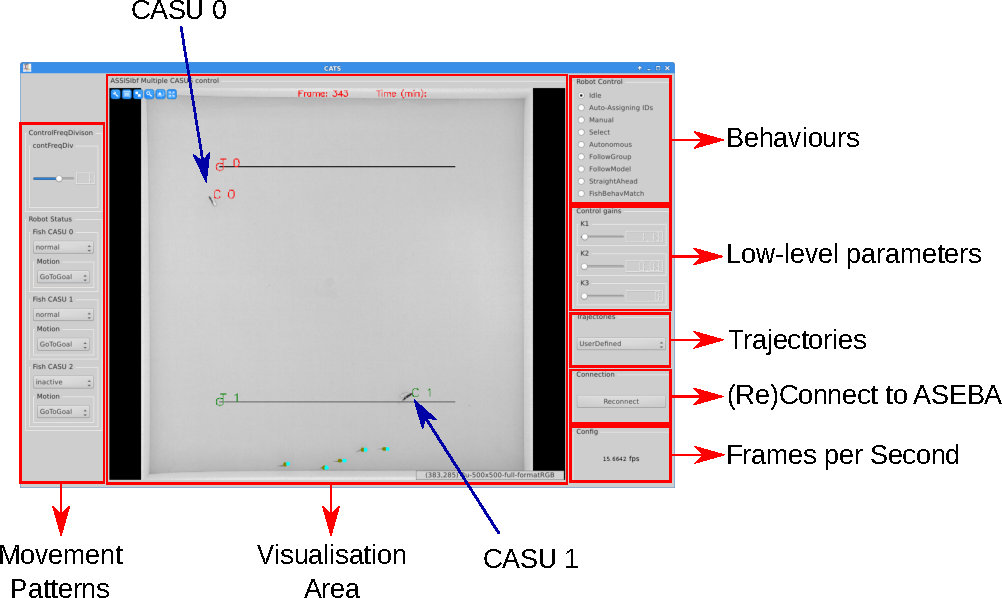
\includegraphics[width=0.75\textwidth]{./figs/GUI-desc}
\caption{Graphical Interface of CATS during a typical experiment. The video stream from the camera is displayed on the visualisation area, at the center panel. Colored disks are placed
on the detected positions of the fish and robots: the tracking system detect the centroids of each agent, and the position of the head of the fish or lures. Big circles of colors are used to represent the positions of the robots. The user can choose current the behaviour and movement pattern of each robot using the controls on the left and right of the visualisation area.}
\label{fig:GUI-desc}
\end{figure}

\begin{figure}[ht]
\centering
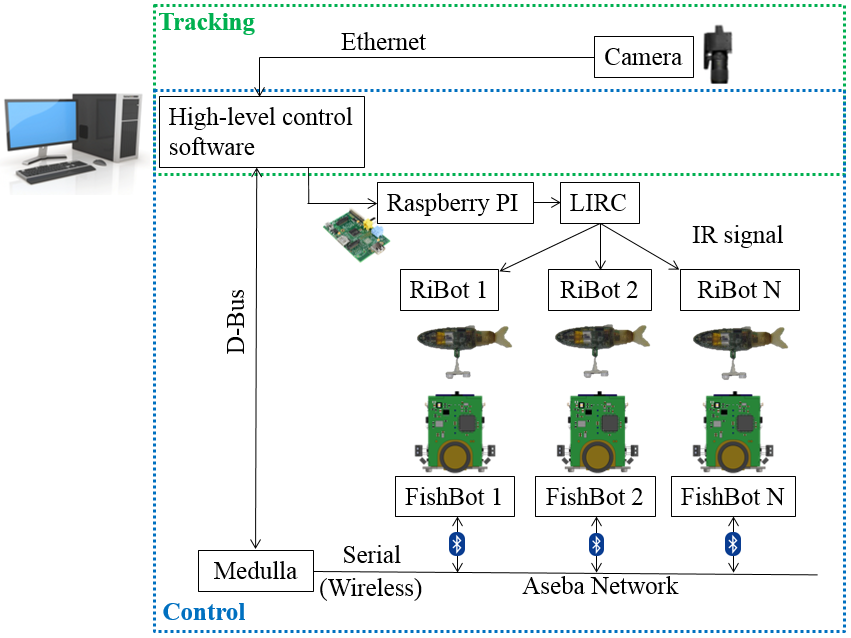
\includegraphics[width=0.75\textwidth]{./figs/ControlArchitecture}
\caption{Architecture of the Fish-CASU vision-based closed-loop control. The high-level control-software tracks each RiBot and fish using frames grabbed by a camera. The same software
is used to control the FishBots' motion as well as RiBots' body movements. For the FishBots, the desired speed of each wheel is sent through a serial connection using Medulla integrated with D-Bus on the ASEBA network, in which all the FishBots are connected and can receive or emit events. For the RiBots, the communication is only one way, where the IR RC5 signal is broadcast to control stepper motors that drive the caudal peduncles.}
\label{fig:ControlArchitecture}
\end{figure}

Different types of behaviours and locomotion patterns were implemented in CATS that the user can either select on a configuration file, or adapt during an ongoing experiment.
The locomotion patterns define how the robot moves while executing selection behaviour.
The following behaviours were implemented:
\begin{itemize}
  \item Local obstacle avoidance
  \item Random walk
  \item Target following : Preprogrammed trajectory or Fish model driven
\end{itemize}

The following motion patterns were implemented:
\begin{itemize}
  \item Constant linear speed
  \item Fish-like patterns
  \item Adaptive fish-like patterns
\end{itemize}

\subsubsection{OS}
All software was written in C++, relied on ICL library for the user interface. It runs under Ubuntu only. 

\subsubsection{Software analysis}
PROS:
\begin{itemize}
  \item Real-time tracker tightly integrated with the robotic control system 
  \item Use of the configuration files to have presets for several experiments
  \item On-line access to the running experiments
\end{itemize}

CONS:
\begin{itemize}
  \item Modularity issues : currently one peace
  \item Flexibility issues : for instance it is not possible to {\it easily} replace one tracking method by another
  \item Scalability issues with the robot's control : not possible to make experiments with tens of robots
  \item The GUI is based on the ICL library that limits drastically its modifications
  \item Poorly commented code
  \item General code quality
      \begin{itemize}
        \item{Memory leaks : variables created but never released}
        \item{unclear (missing?) code conventions}
        \item{some methods are really big, and might be cut in smaller methods (CATApp::robotControl) }
      \end{itemize}
  \item One need to launch {\it asebaswitch} and {\it GStreamer} in addition to CATS to run experiments.
\end{itemize}


\chapter{CATS2.0 design}\label{chap:cats2}

\section {Requirements}
Here we outline the main functional and non-functional requirements for the CATS2 software\footnote{This section was done in May, 2016}.

The goal is to deliver a software that would take into account the strong points of existing solutions and would resolve the known limitations.

\begin{table}[h]
\begin{tabular}{|p{0.25\textwidth}|p{0.75\textwidth}|}
  \hline
  \multicolumn{2}{|c|}{Functional requirements} \\
  \hline
  \multirow{5}{*}{Tracking} & $\bullet$ Possibility to switch between different tracking methods, to add new ones \\
  & $\bullet$ Support of the various cameras (USB video class cameras, Basler cameras is a minimum requirement) \\
  & $\bullet$ Possibility to receive the input video stream from several cameras in the same time \\
& $\bullet$ Write positions of fishes and robots to output files \\
&  $\bullet$ Send positions of fishes and robots to HEAF \\
\hline
  \multirow{3}{*}{Flexible GUI} & $\bullet$ Show the video streams \\
  & $\bullet$ Show the positions of fishes and robots above the video stream \\
  & $\bullet$ Set the parameters of the robots \\
\hline
  \multirow{4}{*}{\parbox{0.25\textwidth}{Multi robot planning and control}} & $\bullet$ Connect automatically to all robots, available on the network, to make the auto discovery of new robots and disconnect robots that are not available anymore \\
  & $\bullet$ Provide the access to each robot's telemetry and parameters (Aseba Studio like) \\
  & $\bullet$ Reliable obstacle avoidance system, ensure that the robot almost never gets stuck in the local minima, provide manual de-blocking  solutions \\
  & $\bullet$ Easy define behavioural strategies based on the areas of the arena \\
\hline
Logging & $\bullet$ Logging system to monitor the software functioning \\
\hline
\end{tabular}
\end{table}

Non-functional requirements:
\begin{itemize}
\item All used libraries must be open source
\item  C++11 / Qt as the base technology
\item  Target systems Linux (minimal), MacOS, Windows
\item  Strict following to coding conventions
\end{itemize}

The following sections present the architecture of the CATS2 software that generally corresponds to the current\footnote{September, 2017} implementation.

\section {The system level design}
The integration of CATS2 with other modules of the robot-fish interaction framework is shown on Fig. \ref{fig:system-level}

\begin{figure}[ht]
\centering
\includegraphics[width=0.99\textwidth]{./outline/system-view-edit}
\caption{Outline of the system level design of CATS2. It receives input streams of one or several cameras, processes them to detect and track robots and animals, stores the resulted trajectories in the log files, control the robots based of the user-defined strategies, and, finally, communicates with the bee setup.}
\label{fig:system-level}
\end{figure}

\section {CATS2 architecture}
Fig. \ref{fig:CATS2-modules} shows the design of the internal structure of CATS2.

\begin{figure}[h]
\centering
\includegraphics[width=0.99\textwidth]{./outline/CATS-view-edit}
\caption{Two principal modules of CATS2 are Tracking and Robot Control.}
\label{fig:CATS2-modules}
\end{figure}

\section {Tracking module of CATS2}
The architecture of the tracking module of CATS2 is presented on Fig. \ref{fig:CATS2-tracking-module}.

\begin{figure}[h]
\centering
\includegraphics[width=0.99\textwidth]{./outline/tracking-module-edit}
\caption{The design of the tracking system. Grabber receives the input frames that are time-stamped and transfered via inter-thread queue to Tracker that detects and tracks agents based on the user-defined tracking strategy (in the configuration file). Tracking Data Manager merges together tracking results coming from different sources (cameras), writes the results to log files, and transfers them further to the Robot Control module. The input streams and tracking resutls are visualized by Viewer.}
\label{fig:CATS2-tracking-module}
\end{figure}

\section {Robot Control module of CATS2}
Fig. \ref{fig:CATS2-tracking-module} shows the architecture of the robot control system.

\begin{figure}[h]
\centering
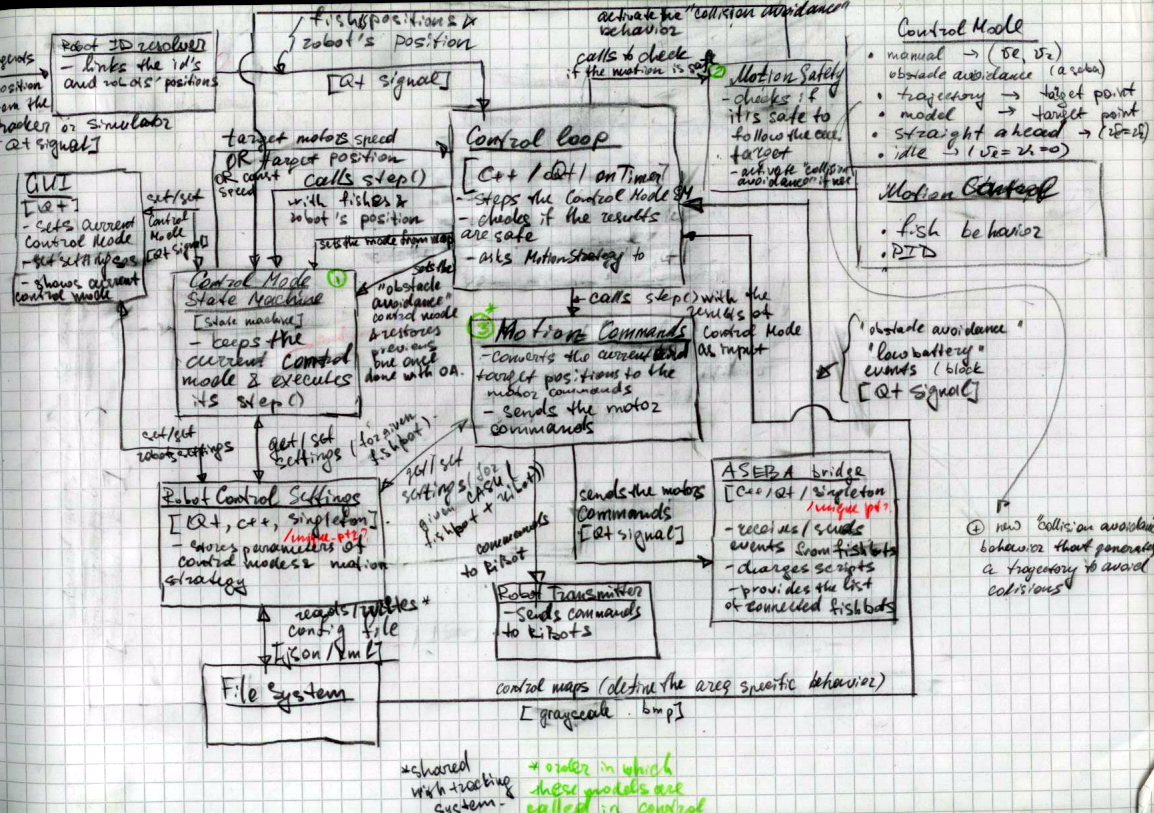
\includegraphics[width=0.99\textwidth]{./outline/robot-control-edit}
\caption{The design of the robot control system. Control Loop executes the current Control Mode that generates the control target (speed or position), and then this control target is converted by Motion Control (or navigation) to the motor commands that are sent to the robot via ASEBA.}
\label{fig:CATS2-robot-control-module}
\end{figure}

\section {Status by September, 2017}
The following functionalities were {\bf not implemented}:
\begin{itemize}
\item Robot Control: the control of the fish robot ({\it ribot})
\item Everywhere: the configuration file is read-only, all the changes in the settings have to be done manually
\end{itemize}

The following functionalities were {\bf implemented differently}:
\begin{itemize}
\item Robot Control: Motion Commands if called {\it navigation}; Motion Safety module is not implemented as a separated unit; control maps are implemented as {\it xml} files and not as grey-scale images. 
\end{itemize}

The following {\bf new} functionalities were implemented:
\begin{itemize}
\item Robot Control: {\it experimental controllers} module that implements experiment specific behaviors combining together various control modes based on the control maps; {\it statistics} module exposes various internal statistics to be available via ZMQ. 
\item {\it Settings interface} allows to modify various internal settings of CATS2 via ZMQ thus allowing the integration of external intelligent systems.
\end{itemize}


\chapter{Environment}\label{chap:Environment}

\section {Source code management}
All source code is managed in a git repository. CATS2 can be found here \url{https://github.com/gribovskiy/CATS2}

\section {Code conventions}
The detailed code conventions can be found in Chapter \ref{chap:code-conventions}.

\section {Target operating system}
Windows and Ubuntu

\section {Compiler}
GCC

\section {Build system}
CMake

\chapter{Code conventions}\label{chap:code-conventions}
\lstset{language=C++} 

\section{Sources}\label{sec:sources}
This is Coding Style: not mandatory, but very useful and pretty to read.

\begin{itemize}
\item  \url{https://wiki.qt.io/Qt_Coding_Style}
\item  \url{https://wiki.qt.io/Coding_Conventions}
\item \url{https://community.kde.org/Policies/Kdepim_Coding_Style}
\item \url{https://wiki.qt.io/API_Design_Principles}
\item \url{https://wiki.qt.io/New_Signal_Slot_Syntax}
\item \url{https://github.com/isocpp/CppCoreGuidelines/blob/master/CppCoreGuidelines.md}
\end{itemize}

% ============================================================================================================================================
\clearpage
\newpage

\section{C++ features}\label{sec:cpp_features}

% === Subsection ====
\subsection{Exceptions}
\begin{itemize}
\item Don't use exceptions
\end{itemize}

% === Subsection ====
\subsection{Casting}
\begin{itemize}
\item If possible, don't use rtti (Run-Time Type Information; that is, the typeinfo struct, the dynamic\_cast or the typeid operators, including throwing exceptions). Use qobject\_cast for QObjects.
\item Avoid C casts, prefer C++ casts (static\_cast, const\_cast, reinterpret\_cast)\footnote{Both reinterpret\_cast and C-style casts are dangerous, but at least reinterpret\_cast won't remove the const modifier}
\item Use the constructor to cast simple types: int(myFloat) instead of (int)myFloat\footnote{When refactoring code, the compiler will instantly let you know if the cast would become dangerous.}
\end{itemize}

% === Subsection ====
\subsection{Templates}
\begin{itemize}
\item Use templates wisely, not just because you can.
\end{itemize}

% === Subsection ====
\subsection{Including headers}
\begin{itemize}
\item In source files, include specialized headers first, then generic headers. Separate the categories with empty lines.
% === START(Example) ====
\begin{lstlisting}[breaklines]
 #include <qstring.h> // Qt class
 
 #include <new> // STL stuff
 
 #include <limits.h> // system stuff
 \end{lstlisting}
% === END(Example) ====
\item If you need to include qplatformdefs.h, always include it as the first header file.
\end{itemize}

% === Subsection ====
\subsection{Operators}
\begin{itemize}
\item The binary operators = (assignment), [] (array subscription),  $\rightarrow$ (member access), as well as the n-ary () (function call) operator, must always be implemented as member functions, because the syntax of the language requires them to. A binary operator that treats both of its arguments equally should not be a member. Because, in addition to the reasons mentioned in the stack overflow answer \footnote{\url{http://stackoverflow.com/questions/4421706/operator-overloading/4421729\#4421729}}, the arguments are not equal when the operator is a member. Example with QLineF which unfortunately has its operator== as a member:
% === START(Example) ====
\begin{lstlisting}[breaklines]
QLineF lineF;
QLine lineN;
 
if (lineF == lineN) // Ok,  lineN is implicitly converted to QLineF
if (lineN == lineF) // Error: QLineF cannot be converted implicitly to QLine, and the LHS is a member so no conversion applies
 \end{lstlisting}
% === END(Example) ====
\end{itemize}
If the operator== was outside of the class, conversion rules would apply equally for both sides.

% === Subsection ====
\subsection{Functions/methods}
\begin{itemize}
\item A function should perform a single logical operation. Keep functions short and simple.
\item If a function is very small and time-critical, declare it inline.
\item  Where there is a choice, prefer default arguments over overloading.
\end{itemize}

% === Subsection ====
\subsection{unsigned int vs. size\_t}
Use size\_t for sizes and indices. The size\_t type is the unsigned integer type that is the result of the sizeof operator (and the offsetof operator), so it is guaranteed to be big enough to contain the size of the biggest object your system can handle\footnote{http://stackoverflow.com/questions/131803/unsigned-int-vs-size-t}.


% === Subsection ====
\subsection{Conventions in Qt source code}
\begin{itemize}
\item Every QObject subclass must have a Q\_OBJECT macro, even if it doesn't have signals or slots, otherwise qobject\_cast will fail.
\item In public header files, always use this form to include Qt headers: \#include <QtCore/qwhatever.h>. The library prefix is neccessary for Mac OS X frameworks and is very convenient for non-qmake projects.
\item Use new signal slot syntax : 
% === START(Example) ====
\begin{lstlisting}[breaklines]
connect(sender, &Sender::valueChanged, receiver, &Receiver::updateValue );
 \end{lstlisting}
% === END(Example) ====
The new syntax can even connect to functions, not just QObjects:
% === START(Example) ====
\begin{lstlisting}[breaklines]
connect(sender, &Sender::valueChanged, someFunction);

connect(sender, &Sender::valueChanged, [=](const QString &newValue) { receiver->updateValue("senderValue", newValue); } );
 \end{lstlisting}
% === END(Example) ====

\end{itemize}

% === Subsection ====
\subsection{Compiler/Platform specific issues}
\begin{itemize}
\item Be extremely careful when using the questionmark operator. If the returned types aren't identical, some compilers generate code that crashes at runtime (you won't even get a compiler warning).
% === START(Example) ====
\begin{lstlisting}[breaklines]
 QString s;
 return condition ? s : "nothing"; // crash at runtime - QString vs. const char *
 \end{lstlisting}
% === END(Example) ====
\item Be extremely careful about alignment. Whenever a pointer is cast such that the required alignment of the target is increased, the resulting code might crash at runtime on some architectures. For example, if a const char * is cast to an const int *, it'll crash on machines where integers have to be aligned at two- or four-byte boundaries.
\item Use a union to force the compiler to align variables correctly. In the example below, you can be sure that all instances of AlignHelper are aligned at integer-boundaries.
% === START(Example) ====
\begin{lstlisting}[breaklines]
union AlignHelper {
     char c;
     int i;
 };
 \end{lstlisting}
% === END(Example) ====
\end{itemize}

\clearpage
\newpage

% ============================================================================================================================================
\section{C++11 features}\label{sec:cpp11_features}

% === Subsection ====
\subsection{auto Keyword}
Optionally, you can use the auto keyword in the following cases: 
\begin{itemize}
\item When it avoids repetition of a type in the same statement.
% === START(Example) ====
\begin{lstlisting}[breaklines]
auto something = new MyCustomType;
auto keyEvent = static_cast<QKeyEvent *>(event);
auto myList = QStringList() << QLatin1String("FooThing") << QLatin1String("BarThing");
 \end{lstlisting}
% === END(Example) ====
\item When assigning iterator types.
% === START(Example) ====
\begin{lstlisting}[breaklines]
auto it = myList.const_iterator();
 \end{lstlisting}
% === END(Example) ====
\end{itemize}

If using auto could make the code less readable, do not use auto; the code is read much more often than written.

% === Subsection ====
\subsection{nullptr}
In C++ code, use nullptr for pointers. 

% === Subsection ====
\subsection{override and final}
\begin{itemize}
 \item Use override that specifies that a virtual function overrides another virtual function. 
 \item Use final that specifies that a virtual function cannot be overridden in a derived class or that a class cannot be inherited from. 
\end{itemize}

% === Subsection ====
\subsection{Objects lifetime management}
\begin{itemize}
 \item Where possible provide a parent object to the objects of classes inheriting QObject, the parent object will take care for the clean up.
 \item Use Qt's smart pointers to manage the pointers. 
\end{itemize} 
  
% === Subsection ====
\subsection{Scoped enums}
Use scoped enums instead of C++98-style enums.



\clearpage
\newpage

% ============================================================================================================================================
% === Chapter ====
\section{Coding style}\label{sec:code_conventions}
\subsection{Indentation}
\begin{itemize}
\item No tabs, 4 Spaces instead of one tab
\item Unix-style linebreaks ('\textbackslash n'), not Windows-style ('\textbackslash r\textbackslash n').
\end{itemize}


% === Subsection ====
\subsection{Declaring variables}

\begin{itemize}
\item  Declare each variable on a separate line
\item  Avoid short or meaningless names
\item  Single character variable names are only okay for counters and temporaries, where the purpose of the variable is obvious
\item  Wait when declaring a variable until it is needed
% === START(Example) ====
\begin{lstlisting}[breaklines]
// Wrong
 int a, b;
 char *c, *d;

 // Correct
 int height;
 int width;
 char *nameOfThis;
 char *nameOfThat;
 \end{lstlisting}
% === END(Example) ====
\item  Variables and functions start with a lower-case letter. Each consecutive word in a variable's name starts with an upper-case letter.
\item  Class members start with {\bf m\_}\footnote{This seems to be inconsistent with the variables naming conventions, to replace my a simple {\bf m}?}. 
% === START(Example) ====
\begin{lstlisting}[breaklines]
 class TableInfo {
  ...
 private:
  string m_tableName;  // OK - starts with m_
};
 \end{lstlisting}
% === END(Example) ====
\item  Data members of structs should be named like ordinary non-member variables, without {m\_} before them.
\item  Avoid abbreviations
% === START(Example) ====
\begin{lstlisting}[breaklines]
 // Wrong
 short Cntr;
 char ITEM_DELIM = ' ';

 // Correct
 short counter;
 char itemDelimiter = ' ';
 \end{lstlisting}
% === END(Example) ====
\item  Classes always start with an upper-case letter. 
\item  Acronyms are camel-cased (e.g. QXmlStreamReader, not QXMLStreamReader).
\end{itemize}

% ==============
% === Subsection ====
\subsection{Whitespace}
\begin{itemize}
\item Use blank lines to group statements together where suited
\item Always use only one blank line
\item Always use a single space after a keyword and before a curly brace:
% === START(Example) ====
\begin{lstlisting}[breaklines]
 // Wrong
 if(foo){
 }

 // Correct
 if (foo) {
 }
 \end{lstlisting}
% === END(Example) ====
\item For pointers or references, always use a single space between the type and '*' or '\&', but no space between the '*' or '\&' and the variable name:
% === START(Example) ====
\begin{lstlisting}[breaklines]
 char *x;
 const QString &myString;
 const char * const y = "hello";
 \end{lstlisting}
% === END(Example) ====
\item Surround binary operators with spaces
\item No space after a cast
\item Avoid C-style casts when possible
% === START(Example) ====
\begin{lstlisting}[breaklines]
 // Wrong
 char* blockOfMemory = (char* ) malloc(data.size());

 // Correct
 char *blockOfMemory = reinterpret_cast<char *>(malloc(data.size()));
 \end{lstlisting}
% === END(Example) ====
\item Do not put multiple statements on one line
\item By extension, use a new line for the body of a control flow statement:
% === START(Example) ====
\begin{lstlisting}[breaklines]
 // Wrong
 if (foo) bar();

 // Correct
 if (foo)
     bar();
 \end{lstlisting}
% === END(Example) ====
\item Use a space after the name of the class
% === START(Example) ====
\begin{lstlisting}[breaklines]
class DbException : public Akonadi::Exception
{
  ...
};
 \end{lstlisting}
% === END(Example) ====
\end{itemize}

% ==============
% === Subsection ====
\subsection{Braces}
\begin{itemize}
\item Use attached braces: The opening brace goes on the same line as the start of the statement. If the closing brace is followed by another keyword, it goes into the same line as well:
% === START(Example) ====
\begin{lstlisting}[breaklines]
 // Wrong
 if (codec)
 {
 }
 else
 {
 }
 
 // Correct
 if (codec) {
 } else {
 }
 \end{lstlisting}
% === END(Example) ====
\item Exception: Function implementations and class declarations always have the left brace on the start of a line:
% === START(Example) ====
\begin{lstlisting}[breaklines]
 static void foo(int g)
 {
     qDebug("foo: %i", g);
 }
 
 class Moo
 {
 };
 \end{lstlisting}
% === END(Example) ====
\item Use curly braces only when the body of a conditional statement contains more than one line:
% === START(Example) ====
\begin{lstlisting}[breaklines]
 // Wrong
 if (address.isEmpty()) {
     return false;
 }
 
 for (int i = 0; i < 10; +''i) {
     qDebug("%i", i);
 }
 
 // Correct
 if (address.isEmpty())
     return false;
 
 for (int i = 0; i < 10;i)
     qDebug("%i", i);
 \end{lstlisting}
% === END(Example) ====
\item Exception 1: Use braces also if the parent statement covers several lines / wraps:
% === START(Example) ====
\begin{lstlisting}[breaklines]
 // Correct
 if (address.isEmpty() || !isValid()
     || !codec) {
     return false;
 }
  \end{lstlisting}
% === END(Example) ====
\item Exception 2: Brace symmetry: Use braces also in if-then-else blocks where either the if-code or the else-code covers several lines:
% === START(Example) ====
\begin{lstlisting}[breaklines]
// Wrong
 if (address.isEmpty())
     qDebug("empty!");
 else {
     qDebug("%s", qPrintable(address));
     it;
 }
 
 // Correct
 if (address.isEmpty()) {
     qDebug("empty!");
 } else {
     qDebug("%s", qPrintable(address));
     it;
 }
 
 // Wrong
 if (a)
     ...
 else
     if (b)
        ...
 
 // Correct
 if (a) {
     ...
 } else {
     if (b)
         ...
 }
 \end{lstlisting}
% === END(Example) ====
\item Use curly braces when the body of a conditional statement is empty
% === START(Example) ====
\begin{lstlisting}[breaklines]
 // Wrong
 while (a);
 
 // Correct
 while (a) {}
 \end{lstlisting}
% === END(Example) ====
\end{itemize}

% ==============
% === Subsection ====
\subsection{Parentheses}
\begin{itemize}
\item  Use parentheses to group expressions:
% === START(Example) ====
\begin{lstlisting}[breaklines]
 // Wrong
 if (a && b || c)
 
 // Correct
 if ((a && b) || c)
 
 // Wrong
 a + b & c
 
 // Correct
 (a + b) & c
 \end{lstlisting}
% === END(Example) ====
\end{itemize}


% ==============
% === Subsection ====
\subsection{Switch statements}
\begin{itemize}
\item  The case labels are in the same column as the switch
\item Every case must have a break (or return) statement at the end or a comment to indicate that there's intentionally no break, unless another case follows immediately.
% === START(Example) ====
\begin{lstlisting}[breaklines]
switch (myEnum) {
 case Value1:
   doSomething();
   break;
 case Value2:
 case Value3:
   doSomethingElse();
   // fall through
 default:
   defaultHandling();
   break;
 }
  \end{lstlisting}
% === END(Example) ====
\end{itemize}


% ==============
% === Subsection ====
\subsection{Jump statements (break, continue, return, and goto)}
\begin{itemize}
\item  Do not put 'else' after jump statements:
% === START(Example) ====
\begin{lstlisting}[breaklines]
 // Wrong
 if (thisOrThat)
     return;
 else
     somethingElse();
 
 // Correct
 if (thisOrThat)
     return;
 somethingElse();
 \end{lstlisting}
% === END(Example) ====
Exception: If the code is inherently symmetrical, use of 'else' is allowed to visualize that symmetry
\item When testing a pointer, use (!myPtr) or (myPtr); don't use myPtr != nullptr or myPtr == nullptr.
\item 
\end{itemize}

% ==============
% === Subsection ====
\subsection{Line breaks}
\begin{itemize}
\item  Keep lines shorter than 100 characters; wrap if necessary
\item  Comment/apidoc lines should be kept below 80 columns
\item  Commas go at the end of wrapped lines; operators start at the beginning of the new lines. An operator at the end of the line is easy to miss if the editor is too narrow.
% === START(Example) ====
\begin{lstlisting}[breaklines]
 // Wrong
 if (longExpression +
     otherLongExpression +
     otherOtherLongExpression) {
 }
 
 // Correct
 if (longExpression
     + otherLongExpression
     + otherOtherLongExpression) {
 }
 \end{lstlisting}
% === END(Example) ====
\item Each member initialization of a method in separate line
% === START(Example) ====
\begin{lstlisting}[breaklines]
class myClass
{
    // some lines
public:
    myClass(int r, int b, int i, int j)
        : r(0)
        , b(i)
        , i(5)
        , j(13)
{
    // more lines
}
};
 \end{lstlisting}
% === END(Example) ====
\end{itemize}

\clearpage
\newpage

% ============================================================================================================================================
\section{Design principles}\label{sec:design}
% === Subsection ====
\subsection{Pointers vs. References}
Most C++ books recommend references whenever possible, according to the general perception that references are "safer and nicer" than pointers. In contrast, Qt Software tends to prefer pointers because they make the user code more readable:
% === START(Example) ====
\begin{lstlisting}[breaklines]
 color.getHsv(&h, &s, &v);
 color.getHsv(h, s, v);
 \end{lstlisting}
% === END(Example) ====
Only the first line makes it clear that there's a high probability that h, s, and v will be modified by the function call.

% === Subsection ====
\subsection{Passing by const-ref vs. Passing by value}
\begin{itemize}
\item If the type is bigger than 16 bytes, pass by const-ref.
\item If the type has a non-trivial copy-constructor or a non-trivial destructor, pass by const-ref to avoid executing these methods.
\item All other types should usually be passed by value.
\end{itemize}


% === Subsection ====
\subsection{Ownership}
We try to get rid of the manual memory management. For this reason
\begin{itemize}
\item In the GUI classes we use the Qt mechanism of ownership.
\item In data classes, handler classes\footnote{The handler classes make a link between the data classes and GUI.} and other classes inheriting QObject we use the Qt's smart pointers, that are provided QObject::deleteLater as destruction mechanism.
\item In all other cases we use smart pointers or references. 

\end{itemize}


\clearpage
\newpage

% ============================================================================================================================================
\section{General Naming Rules}\label{sec:naming_rules}
% === Subsection ====
\subsection{Naming Enum Types and Values}
When declaring enums, we must keep in mind that in C++ (unlike in Java or C\#), the enum values are used without the type:
% === START(Example) ====
\begin{lstlisting}[breaklines]
 namespace Qt
 {
 enum Corner { TopLeft, BottomRight, ... };
 enum CaseSensitivity { Insensitive, Sensitive };
 ...
 };
 
 tabWidget->setCornerWidget(widget, Qt::TopLeft);
 str.indexOf("$(QTDIR)", Qt::Insensitive);
 \end{lstlisting}
% === END(Example) ====

In the last line, what does Insensitive mean? One guideline for naming enum types is to repeat at least one element of the enum type name in each of the enum values:
% === START(Example) ====
\begin{lstlisting}[breaklines]
 namespace Qt
 {
 enum Corner { TopLeftCorner, BottomRightCorner, ... };
 enum CaseSensitivity { CaseInsensitive,
 CaseSensitive };
 ...
 };
 
 tabWidget->setCornerWidget(widget, Qt::TopLeftCorner);
 str.indexOf("$(QTDIR)", Qt::CaseInsensitive);
 \end{lstlisting}
% === END(Example) ====

% === Subsection ====
\subsection{Naming Boolean Getters, Setters, and Properties}
\begin{itemize}
\item Adjectives are prefixed with is-. Examples: isChecked(), isDown(), isEmpty(), isMovingEnabled(), 
\item However, adjectives applying to a plural noun have no prefix: scrollBarsEnabled(), not areScrollBarsEnabled()
\item Verbs have no prefix and don't use the third person (-s): acceptDrops(), not acceptsDrops()
\item The getter for the class' member "\_foobar", would be called "foobar()" (not "getFoobar()")
\item Nouns generally have no prefix:  autoCompletion(), not isAutoCompletion(); sometimes, having no prefix is misleading, in which case we prefix with is-:
isOpenGLAvailable(), not openGL()
\end{itemize}

The name of the setter is derived from that of the getter by removing any is prefix and putting a set at the front of the name; for example, setDown() and setScrollBarsEnabled(). The name of the property is the same as the getter, but without the is prefix.

% === Subsection ====
\subsection{Naming files}
Like in Boost we use .h/.c for C files and .hpp/.cpp for the C++ files.

\clearpage
\newpage
% ============================================================================================================================================
\section{Recommended compiler flags}\label{sec:compiler_flags}
-std=c++11 -Wall -Wextra -Wcast-align -Wcast-qual -Wdisabled-optimization -Wformat=2 -Wlogical-op -Wmissing-declarations -Wmissing-include-dirs -Wnoexcept -Woverloaded-virtual -Wredundant-decls -Wstrict-null-sentinel -Wstrict-overflow=5 -Wswitch-default -Wno-unused-parameter -Wold-style-cast -Wnull-dereference -Wsuggest-override -Wsuggest-final-methods -Wfloat-equal -Wundef -Wshadow

In debug mode we activate the AddressSanitizer fill the following flags : -fsanitize=address -fsanitize=thread -fsanitize=undefined

\clearpage
\newpage
% ============================================================================================================================================
\section{Artistic Style (astyle) automatic code formatting}\label{sec:astyle}
You can use astyle (>=1.23) to format code or to test if you have followed this document. Run the following command:
% === START(Example) ====
\begin{lstlisting}[breaklines]
astyle --indent=spaces=4 --brackets=linux \
       --indent-labels --pad=oper --unpad=paren \
       --one-line=keep-statements --convert-tabs \
       --indent-preprocessor \
       `find -type f -name '*.cpp'-or -name '*.hpp'`
 \end{lstlisting}
% === END(Example) ====

With astyle (>=2.01) you need to run the following command:
% === START(Example) ====
\begin{lstlisting}[breaklines]
astyle --indent=spaces=4 --brackets=linux \
       --indent-labels --pad-oper --unpad-paren --pad-header \
       --keep-one-line-statements --convert-tabs \
       --indent-preprocessor \
       `find -type f -name '*.cpp' -or -name '*.hpp'`
 \end{lstlisting}
% === END(Example) ====

Note: With more recent astyle --brackets has become --style, so change --brackets=linux to --style=linux.

\clearpage
\newpage
% ============================================================================================================================================
\section{Git commit messages}\label{sec:versioning}
We suggest to use the template provided here: 
\begin{itemize}
\item  \url{http://codeinthehole.com/writing/a-useful-template-for-commit-messages/}
\item  \url{http://chris.beams.io/posts/git-commit/}
\end{itemize}



\end{document}

